%%%%%%%%%%%%%%%%%%%%%%%%%%%%%%%%%%%%%%%%%%%%%%%%%%%%%%%%%%%%%%%%%%%%%%%%%%%%%%%%%%
%%																				%%
%% File name: 		20hannes.tex												%%
%% Project name:	Hochleistungsantenne										%%
%% Type of work:	T3X00 project work											%%
%% Author:			Sarah Brückner, Maximilian Stiefel, Hannes Bohnengel		%%
%% Date:			13th May 2016												%%
%% University:		DHBW Ravensburg Campus Friedrichshafen						%%
%% Comments:		Created in gedit with tab width = 4							%%
%%																				%%
%%%%%%%%%%%%%%%%%%%%%%%%%%%%%%%%%%%%%%%%%%%%%%%%%%%%%%%%%%%%%%%%%%%%%%%%%%%%%%%%%%

\chapter{GPredict}

\section{Übersicht}

GPredict ist eine freie Software zur Satellitenverfolgung und Orbitvorhersage und steht als Quellcode oder bereits fertig kompiliertes Programm für Windows, Mac OS und Linux zur Verfügung. Die Software ist in C geschrieben und unter der GNU \ac{GPL} lizenziert, somit kann sie frei verändert und an die entsprechenden Nutzervoraussetzungen angepasst werden.\newpar
In Abbildung \ref{fig:gpredict-principle} ist das Prinzip eines Satellitenverfolgungsprogramms zu sehen (die blauen Blöcke stellen hierbei die Funktionalität des Programms dar). Zunächst wird an Hand der Keplerschen Bahnelemente und dem aktuellen Zeitpunkt die absolute Position des Satelliten berechnet. Daraufhin wird der Vektor, der von der Bodenstation zum Satelliten zeigt, bestimmt. Nun können Azimut und Elevation dieses Vektors für die Ansteuerung der Antenne verwendet werden.

\begin{figure}[h]
	\centering
	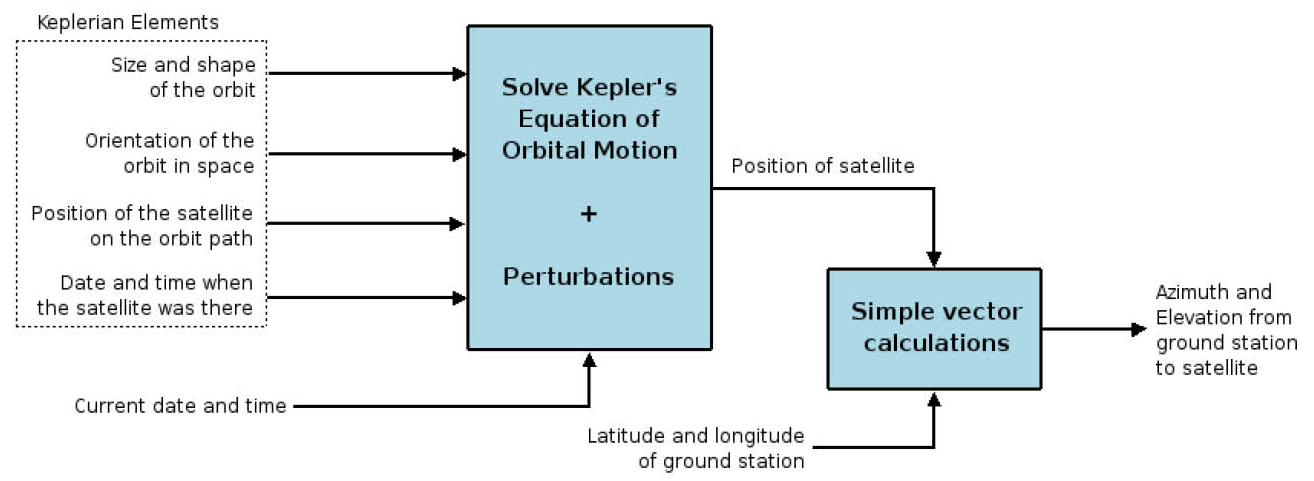
\includegraphics[width=1\textwidth]{gpredict-principle}
	\caption{Prinzip eines Satellitenverfolgungsprogramms \cite{gpredictmanual}}
	\label{fig:gpredict-principle} 
\end{figure}

Zur Berechnung der Satellitenposition wird auf den NORAD SGP4/SDP4 Algorithmus zurückgegriffen (siehe Abschnitt XXX). Um hierfür zu jedem Zeitpunkt die aktuellen Kepler-Elemente des zu verfolgenden Satelliten zu kennen, gibt es unter GPredict die Möglichkeit einer automatischen Aktualisierung über HTTP, FTP oder aus dem lokalen Verzeichnis.

\clearpage

Bei GPredict ist im Gegensatz zu anderen Satellitenverfolgungsprogrammen wie SatPC32 kein Limit an zu verfolgenden Satelliten und Bodenstationen gegeben. Durch die Verwendung von Modulen kann außerdem unkompliziert zwischen verschiedenen Konfigurationen gewechselt werden. Die Orbitvorhersage eines Satelliten lässt sich sowohl grafisch als auch tabellarisch darstellen, wobei durch die Einstellungen verschiedenster Parameter eine sehr individuelle Anzeige erreicht werden kann \cite{gpredictsource}.

\section{Grafische Oberfläche}

In Abbildung \ref{fig:gpredictstartup} ist die grafische Oberfläche von GPredict zu sehen. In der Standardkonfiguration ist dort zunächst die Kartenansicht bzw. Map View (oben), die Polaransicht bwz. Polar View (links unten) und die Einzelsatellitenansicht bzw. Single-Satellite View (rechts unten) zu sehen.

\begin{figure}[h]
	\centering
	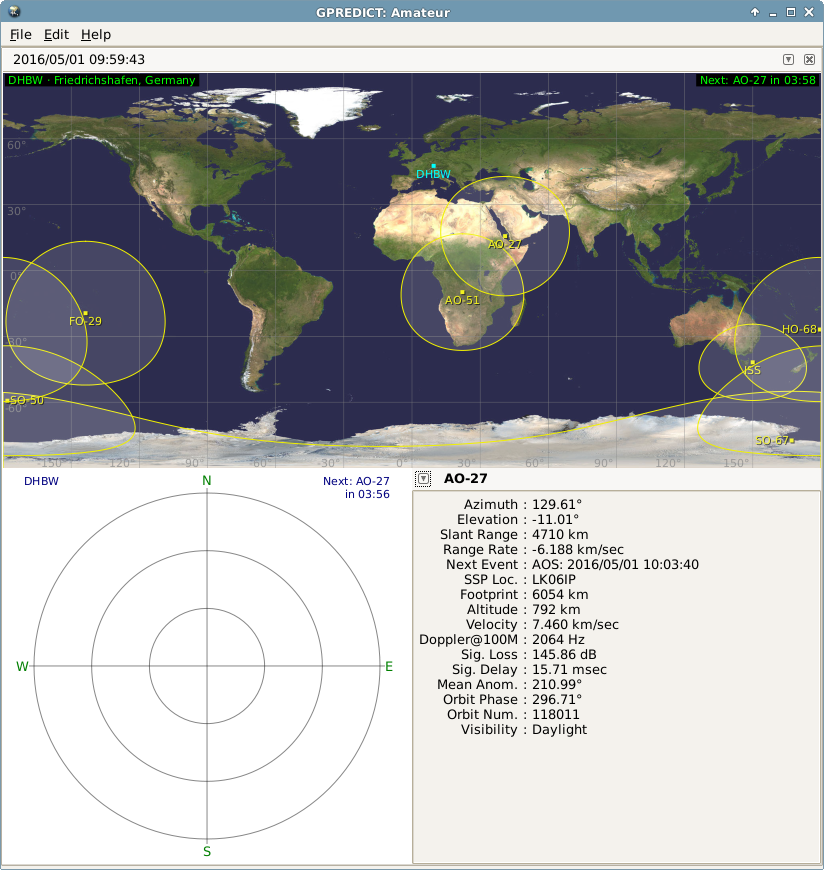
\includegraphics[width=0.75\textwidth]{gpredict-startup.png}
	\caption{Standardoberfläche von GPredict}
	\label{fig:gpredictstartup} 
\end{figure}

\clearpage

Im Folgenden werden die verschiedenen, möglichen Ansichten genauer beschrieben:\\
. \hspace{3cm}\textbf{!!! Evtl. ohne itemize !!!}

\begin{itemize}
	\parskip0pt
	\item \textbf{Map View:}
	\item \textbf{Polar View:}
	\item \textbf{Single-Satellite View:}
	\item \textbf{List View:}
	\item \textbf{Upcoming Passes View:}
	\item \textbf{Module Pop-Up Menu}
	\begin{itemize}	
		\item \textbf{Antenna Control (Rotoren):}
		\item \textbf{Radio Control}
		\item \textbf{Sky at a Glance:}
		\item \textbf{Time Controller:}
		\item \textbf{Modul-Einstellungen (Configure):}
	\end{itemize}
\end{itemize}

\clearpage

\section{HamLib-Programmierschnittstelle}



\begin{figure}[h]
	\centering
	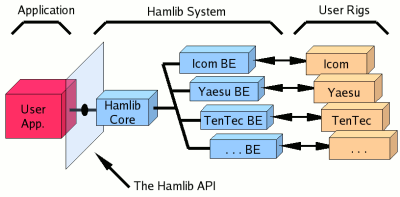
\includegraphics[width=0.5\textwidth]{hamlib}
	\caption{HamLib Design \cite{hamlib}}
	\label{fig:hamlib} 
\end{figure}

\clearpage

\section{Inbetriebnahme unter Windows}

Dieser Text soll ein Test sein, ob die .tex File auch online bearbeitet werden kann.

\section{Inbetriebnahme unter Linux}
